%# -*- coding: utf-8-unix -*-
%% ============================================================================
%% main.tex
%% ============================================================================

\documentclass{scutthesis}

\school{电子与信息学院}
\major{信息工程}
\studentname{某某某}
\studentid{201500000000}
\advisor{某某某教授}
\theistitle{基于卷积神经网络的手写数字及写字人识别}
\submitdate{2019 年 3 月 26 日}
\chinesekeywords{多变量系统; 预测控制; 环境试验设备}
\englishkeywords{Writer recognition;Convolutional Neural Network;Handwritten character recognition}
\addbibresource{bib/thesis.bib}

\begin{document}
  \makecover

  \frontmatter
  \begin{abstract}
    炔烃和叠氮化合物的点击化学反应,有着快速、百分百原子利用率、产物高选择
    性等众多优点,被誉为点击化学中的精华。基于此反应拓展而来的点击聚合反应,迅
    速在高分子材料领域获得了了广泛关注和应用。

    ......
    
    我们还尝试了采用不同单体,在最优条件下进行反应,均获得了高分子产物。表
    明了该反应体系的普适性。

  \end{abstract}
  \begin{englishabstract}
    Artificial Neuron Network (ANN) simulates human being’s brain 
    function and build the network structure. Convolutional Neural 
    Network (CNN) have many advantage, such as ...... 
    
    (2) This paper introduces the common pretreatment method of image, 
    such as collecting image, normalization, graying and binarization. 
    And apply these to the handwritten numeral recognition experiment 
    and handwritten numerals writer recognition experiments.
  \end{englishabstract}
  
  \tableofcontents

  \mainmatter
  \chapter{绪论}
\section{引言}

当今社会,科技的飞速发展为大家􏲁供了快捷与舒适,但与此同时也增添了在信
息安全上的危险。在过去的二十几年来,我们通过数字密码来鉴别身份,但是随着科
技的发展,不法分子借用高科技犯罪的案例年年增高,密码被盗的情况时常发生。因
此,怎样科学准确的辨别每一个人的身份则成为当今社会的重要问题。

\section{研究背景}
随着科技的日益发展,传统的密码因为记忆的繁琐以及容易被盗,似乎已经不再 
能满足这个通信发达的社会的需求。人们急需一种更便捷而且辨识度更高的方式来辨 
识身份。循着便捷与辨识度高这两个约束条件 \cite{ELIDRISSI94},我们联想到
的便是存在于每个人身上的生物特征,所以基于每个人身上不同的生物特征而研究的
鉴别技术现在成为了身份辨别技术上的主流。

\section{研究现状}
笔迹 \cite{imgprocesszh} 获取的方式有两种,所以鉴别方式也分为离线鉴别
和在线鉴别 \cite{lecun1998gradient}。在线鉴别是采用专用的数字板来实时
收集书写信号。由文献\parencite{RManual,kocher99,chen2007ewi} 可知,
因为信号是实时采集的,所以能采集的数据不仅包括笔迹序列,而且可以采集到书写时
的加速度、压力、速度等丰富有用的动态信息。

\section{论文结构}
本文分为四章。其中第一章简述了笔迹识别的研究背景和意义以及笔迹识别的基
础知识等。第二章节从卷积神经网络的发展历史、网络结构、学习规律三方面详细的
讲述了卷积网络的基础知识。第三章针对本文中的手写数字及写字人实验具体设计卷
积神经网络的网络结构以及训练过程。第五章节是手写数字识别及写字人识别实验的
结果与分析。
  \chapter{卷积神经网络的基础知识}
\section{卷积神经网络的网络结构}
卷积神经网络作为深度学习的一个分支,在网络结构上同样含有深度学习的“深
度”性。网络拓扑结构是一个多层的神经网络[7],网络的每一层由多个独立的
神经元组 成的二维平面组成。网络一般分为输入层、卷积层、池化层、全连接
层、输出层等 \cite{tiledsets}。

\subsection{输入层}
因为卷积神经网络可以直接的接受二维的视觉模式[8],所以我们可以直接把简单预
处理后的二维图像输入到输入层中。
% \cite{2014wangqiang}

\subsection{输出}
......

\section{神经网络的学习规律}
如果用 $l$ 来表示当前的网络层,那么当前网络层的输出如公式 \ref{eq:networkoutput} 所示:

\begin{equation}
  \label{eq:networkoutput}
  x^l=f(u), \text{其中} u'=mathbf{W}^l x^{l-1}+b^l
\end{equation}
  
%# -*- coding: utf-8-unix -*-
% !TEX program = xelatex
% !TEX root = ../main.tex
% !TEX encoding = UTF-8 Unicode
%%==================================================
%% chapter04.tex for SCUT Thesis
%% based on SJTUThesis
%% modified by Phree
%% Encoding: UTF-8
%%==================================================

\chapter{手写数字及写字人识别实验过程及其结果}
\section{手写字体识别实验}
\subsection{样本简介}
本论文的手写数字识别实验当中所用的样本分为两类,一类是训练样本集,另一类是测试样本集。

实验当中的训练样本集采用的是手写数字 MNIST 数据库\parencite{DPMG,kocher99,cnproceed}。这个数据库当中包含训练集样本 60000 个样例和测试集样本 10000 个样例。MNIST 数据库当中的数字样本已 经全部大小归一化灰度化并且集中到同一个固定大小的图像当中。该数据库包括 MST 的 SD-1 和 SD-3 数据库,当中包含一系列的二级制的手写数字图像。其中 SD-1 的收 集者来源是某高中的在校学生,而 SD-3 是由人口调查局员工收集的。则我们的训练样 本集也就是 MNIST 当中的训练样本集有 30000 个样本来自 SD-3,而另外 30000 个样 本来自 SD-1。这 60000 个训练样本分别来自约 250 个采集者。
\subsection{Writer Depend类数字识别实验}
\subsubsection{ABCvsA数字识别实验}
实验内容:以A写字人、B写字人和C写字人,合计3000个数字0到9的数字图像数据为训练样本集。A写字人的1000个数字0到9的数字图像数据为测试样本集。学习率为1,单次训练样本数为10个,共训练40次。若识别所得数字与给定的标签匹配,则视为正确;不匹配则视为错误。

\begin{table}[!hpb]
  \centering
  \caption[指向一个表格的表目录索引]
    {ABCvsA 数字识别实验结果}
  \label{tab:firstone}
  \begin{tabular}{C{8em}|C{4em}|C{10em}|C{6em}} \hline
    训练样本 & ABC     & 样本个数      & 3000 \\ \hline
    测试样本 & A       & 样本个数      & 1000 \\ \hline
    训练次数 & \void   & 单次训练样本数 & 10   \\ \hline
    学习率   & 1       & 正确率        & 99.50\% \\ \hline
  \end{tabular}
\end{table}

\subsubsection{ABCvsABC 数字识别实验}

实验内容:以 A 写字人、B 写字人和 C 写字人,合计 3000 个数字 0 到 9 的数字 图像数据为总样本集。在总样本集当中随机抽取 2400 个为训练样本集,余下的 600 个 为测试样本集。学习率为 1,单次训练样本数为 10 个,共训练 40 次。若识别所得数字 与给定的标签匹配,则视为正确;不匹配则视为错误。

\begin{table}[!hpb]
  \centering
  \caption[指向一个表格的表目录索引]
    {ABCvsABC 数字识别实验结果}
  \label{tab:firstone}
  \begin{tabular}{C{8em}|C{4em}|C{10em}|C{6em}} \hline
    训练样本 & ABC     & 样本个数      & 2400     \\ \hline
    测试样本 & A       & 样本个数      & 600      \\ \hline
    训练次数 & 40      & 单次训练样本数 & 10       \\ \hline
    学习率   & 1       & 正确率        & 92.00\% \\ \hline
  \end{tabular}
\end{table}

\subsection{WriterDepend 类数字识别实验结果分析}

下面我们选取 Writer Depend 类数字识别实验当中的两个典型的例子 ABCvsA 数字识别实验以及 MNIST\&ABCvsA 数字识别实验的结果做详细分析。我们从 ABCvsA 数字识别实验中的训练样本集和测试样本集的手写数字图像样本集当中分别随机抽取一幅图像如图 4-1 所示。

\begin{figure}[!htp]
  \centering
  \subcaptionbox{实验训练集\label{fig:epspdf:a}} %标题的长度,超过则会换行,如下一个小图。
    {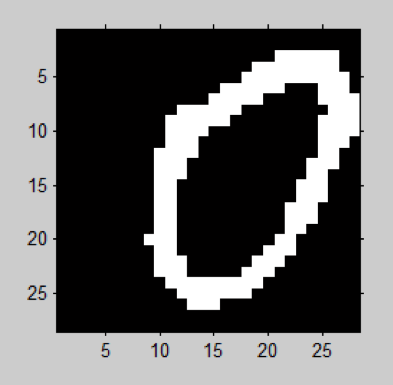
\includegraphics[height=6cm]{figure/experiment1.png}}
  \hspace{4em}
  \subcaptionbox{实验测试集\label{fig:epspdf:b}}
    {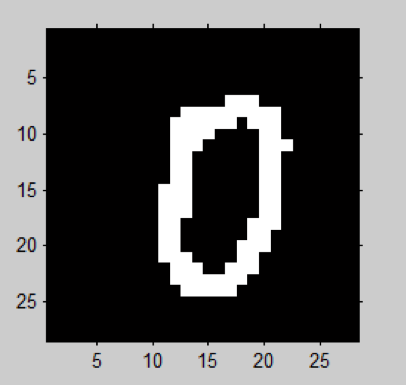
\includegraphics[height=6cm]{figure/experiment2.png}}
  \caption{ABCvsA 数字识别实验集}
  \label{fig:pdfeps-subcaptionbox}
\end{figure}

下面我们对上述的训练集和测试集进行 40 次学习率为 2,单次训练样本为 10 的迭 代,得到错误率为 0.50%,而其中每次训练时的误差值组成的历史误差值画图分析如 下:

......

\subsection{WriterIndepend类数字识别实验}
实验内容:以 MNIST 数据库为训练样本集,共计 60000 个训练样本。以 A 写字 人合计 1000 个数字 0 到 9 的数字图像数据为测试样本集写字人识别实验

......

\subsection{两位写字人识别实验}
\subsubsection{单个数字的写字人识别实验}

实验内容:以 A 写字人,合计 800 个数字 5 的数字图像数据加上 B 写字人,合计 800 个数字 5 的数字图像数据,共计 1600 个样本为总样本集。随机选取其中的 1200 个 样本为训练样本集,其余的 400 个样本为测试样本集。学习率为 2,单次训练样本数为 10 个,共训练 30 次。若识别所得写字人与给定的标签匹配,则视为正确;不匹配则视 为错误。

\begin{table}[!hpb]
  \centering
  \caption[指向一个表格的表目录索引]
    {单个数字写字人识别实验结果}
  \label{tab:firstone}
  \begin{tabular}{C{8em}|C{4em}|C{10em}|C{6em}} \hline
    训练样本 & A5\&B5  & 样本个数      & 1200 \\ \hline
    测试样本 & A5\&B5  & 样本个数      & 400 \\ \hline
    训练次数 & 30      & 单次训练样本数 & 10   \\ \hline
    学习率   & 2       & 正确率        & 99.75\% \\ \hline
  \end{tabular}
\end{table}

\subsubsection{单个数字的写字人识别实验结果分析}
......

\section{本章小结}
......。
 

  \printbibliography[heading=bibintoc]

  \begin{thanks}
    感谢所有测试和使用交大学位论文 LATEX 模板的同学! 
    
    感谢那位最先制作出博士学位论文 LATEX 模板的交大物理系同学!
    
    感谢 William Wang 同学对模板移植做出的巨大贡献!
    
    感谢 @weijianwen 学长一直以来的开发和维护工作!
    
    感谢 @sjtug 以及 @dyweb 对 0.9.5 之后版本的开发和维护工作! 
    
    感谢所有为模板贡献过代码的同学们, 以及所有测试和使用模板的各位同学!
  \end{thanks}
 \end{document}